\documentclass[border=3mm]{standalone}
\usepackage{tikz}
\usetikzlibrary{circuits.logic.US}

\begin{document}
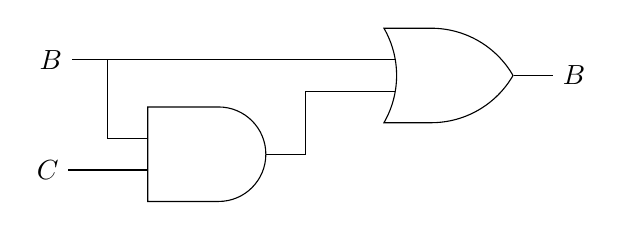
\begin{tikzpicture}[circuit logic US,
                    tiny circuit symbols,
                    every circuit symbol/.style={fill=white,draw,logic gate input sep=4mm, logic gate inverted radius=1mm}
]

\node [and gate, inputs = nn] at (0,0) (and1) {};
\node [or gate, inputs = nn] at ($(and1) + (3.0cm,1)$) (or1) {};
\draw (or1.input 1) -- ++(left:41mm) node[left] (B) {$B$};
\draw (and1.input 1) -- ++(left:5mm) |- (or1.input 1);
\draw (and1.input 2) -- ++(left:10mm) node[left] (C) {$C$};
\draw (and1.output) -- ++(right:5mm) |- (or1.input 2);
\draw (or1.output) -- ++(right:5mm) node[right] (Y) {$B$};
%
\end{tikzpicture}
\end{document}
